In the same way that \enquote{to add} is \fillin[to sum], to multiply is to calculate the \fillin[product].

Much in the same way that we \emph{visualised} addition, we are able to visualise multiplication:

\begin{figure}[ht]
    \label{fig:m1}
    \centering
    
\begin{tikzpicture}
        \foreach \x in {0,1,...,4}
        \foreach \y in {0,1,2}
        \filldraw (\x,\y) circle (0.1);
    \end{tikzpicture}
    \caption{$3\times 5 = 15$ }
\end{figure}

In mathematics, one thing you must reconcile with as early as possible is the fact that 1 concept can be understood, or thought of, in multiple different ways; and each of these ways provides different value. 
For example: multiplication can be conceptualised as addition!

\begin{figure}[ht]
    \label{fig:m2}
    \centering
    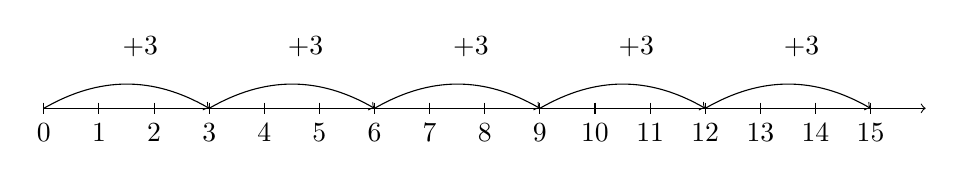
\begin{tikzpicture}[scale=0.7]
        \draw[->] (0,0) -- (16,0);
        \foreach \x in {0,1,...,15}
            \draw[shift={(\x,0)}] (0,3pt) -- (0,-3pt) node[below] {$\x$};
        \foreach \x in {0,3,...,12}
            \draw[->] (\x,0) to[bend left] (3+\x,0) node [above left=15pt] {$+3$};
    \end{tikzpicture}

    \caption{$5\times 3$}
\end{figure}

Note that in the Figure~\ref{fig:m2}, we've demonstrated $5\times 3$ as opposed to the equation we've been thinking about: $3\times 5$. Why is are these 2 the same thing?
\begin{solutionordottedlines}[1in]
    The property of commutativity that we studied in the last lesson, applies to the multiplication operator!
\end{solutionordottedlines}

\fbox{
    \centering
    \parbox{\linewidth}{
        {\large \textbf{Note:} Associativity also applies to multiplication.\[(a\times b)\times c = a \times (b\times c)\]}
}
}

\subsection{Tricks of the Trade}
\subsubsection{Multiplication with 0}
This concept is elementary, but important:

\fbox{
    \centering
\textsc{anything multiplied by 0 is equal to 0}}

\subsubsection{Multiplication by powers of 10}
This is straight-forward---look at how many 0's the power of 10 has, and then just give all those 0's to the other operand\footnote{you should use the space in the margins to define this word if you do not know what it means!}

Thus, $2\times 10$ will just mean I take 1 zero to the 2: $20$. $90\times 1000$ means I take 3 zeros to the $90\,\leadsto\, 90,000$.

\begin{tabular}{lr}
    $2\times 100 =$\fillin[200] & $32\times 10 =\fillin[320]$\\[0.4cm]
    $2\times 1000 = \fillin[2000]$ & $32\times 10000 = \fillin[320000]$\\[0.4cm]
    $2\times 10 = \fillin[20]$ & $32 \times 1000 = \fillin[32000]$
\end{tabular}

\begin{exercises}
    There are no examples this time, you'll be fine. You have 6 minutes:
    \begin{questions}
        \Question[7] Perform each multiplication
        \begin{multicols}{2}
        \begin{parts}
            \part \(23 \times 0=\fillin[0]\)
            \part \(33 \times 1=\fillin[33]\)
            \part \(43 \times 10=\fillin[430]\)
            \part \(73 \times 100=\fillin[7300]\)
            \part \(93 \times 1000=\fillin[93000]\)
            \part \(17 \times 10=\fillin[]\)
            \part \(89 \times 0=\fillin[]\)
            \part \(100 \times 1=\fillin[]\)
            \part \(120 \times 100=\fillin[]\)
            \part \(18 \times 1000=\fillin[]\)
            \part \(100 \times 100=\fillin[]\)
            \part \(1000 \times 73=\fillin[]\)
            \part \(10000 \times 100=\fillin[]\)
            \part \(67430 \times 1000=\fillin[]\)
        \end{parts}
        \end{multicols}
        \Question[] Carry out each calculation, using associativity property for multiplication.\\
        \begin{parts}
            \begin{multicols}{2}
            \part \(25 \times 4 \times 6=\fillin[]\)
            \part \(5 \times 26 \times 2=\fillin[]\)
            \part \(50 \times 49 \times 2=\fillin[]\)
            \part \(5 \times 43 \times 20=\fillin[]\)
            \part \(16 \times 5 \times 40=\fillin[]\)
            \part \(1 \times 34 \times 20=\fillin[]\)
            \part \(13 \times 6 \times 0=\fillin[]\)
            \part \(6 \times 10 \times 10 \times 2=\fillin[]\)
            \end{multicols}
        \end{parts}
        \question Fill in each box with a number to make the statements true.
        \begin{parts}
            \Part[1] \((3 \times 2) \times 7=3 \times(\square \times 7)\)
            \Part[1] \((5 \times 9) \times(2 \times 8)=9 \times 8 \times(\square \times 2)\)
        \end{parts}
        \Question[2] Ian has 13 jars, each containing 20 olives. If he decides to redistribute the olives equally among 20 jars, how many olives will there be in each jar?
            \begin{solutionorbox}[1in]
            \end{solutionorbox}
        \Question[2] Six friends buy a large box of jelly snakes. The snakes come in 5 different colours. How many snakes are needed so that every person has two of each colour?
            \begin{solutionorbox}[1in]
            \end{solutionorbox}
        \Question[2] Bricks are arranged on a concrete floor in 12 rows of 25, and stacked 4 bricks high. How many bricks are there in total?
            \begin{solutionorbox}[1in]
            \end{solutionorbox}
        \Question[2] Holly has prepared 28 bags of lollies for her birthday party. Each bag has 9 lollies in it. She makes these into 14 new bags when some of her friends do not turn up. How many lollies will each person now receive?
            \begin{solutionorbox}[1in]
            \end{solutionorbox}
    \end{questions}
\end{exercises}
